\documentclass[8pt, a4paper, oneside, twocolumn]{extarticle}
\usepackage{graphicx}
\usepackage[export]{adjustbox}
\usepackage[compact]{titlesec}  % documentation: http://mirror.iopb.res.in/tex-archive/macros/latex/contrib/titlesec/titlesec.pdf  
\usepackage{kotex}
\usepackage[left=0.8cm, right=0.8cm, top=2cm, bottom=0.3cm, a4paper]{geometry}
\usepackage{amsmath}
\usepackage{ulem}
\usepackage{amssymb}
\usepackage{minted}  % syntax highlighting
\usepackage{enumitem}
\setlist{nolistsep}
\usepackage{fancyhdr} % documentation: http://ctan.math.utah.edu/ctan/tex-archive/macros/latex/contrib/fancyhdr/fancyhdr.pdf
\usepackage{lastpage}  % just so that we can use \pageref {LastPage}
\usepackage{color, hyperref}
% The lines in the table of contents become links to the corresponding pages in the document by simply adding in the preamble of the document the line
\usepackage{tikz}
\usetikzlibrary{positioning,chains,fit,shapes,calc}
\newcommand{\swastik}[1]{%
    \begin{tikzpicture}[#1]
        \draw (-1,1)  -- (-1,0) -- (1,0) -- (1,-1);
        \draw (-1,-1) -- (0,-1) -- (0,1) -- (1,1);
    \end{tikzpicture}%
}
\newcommand{\revised}{To be \textcolor{red}{\textbf{revised}}.}
\titlespacing*{\section}
{0pt}{0px plus 1px minus 0px}{-2px plus 0px minus 0px}
\titlespacing*{\subsection}
{0pt}{0px plus 1px minus 0px}{0px plus 3px minus 3px}
\titlespacing*{\subsubsection}
{0pt}{0px plus 1px minus 0px}{0px plus 3px minus 3px}
\setlength{\columnseprule}{0.4pt}
\DeclareRobustCommand{\stirling}{\genfrac\{\}{0pt}{}}
\setlength{\parindent}{0pt}  % so that there is no indent of paras.
\setminted{breaklines=true, tabsize=2, breaksymbolleft=}
\begin{document}
\pagenumbering{arabic}
\title{\swastik {scale = 0.2} {}DBMS Short Revision Notes{} \swastik {scale = 0.2}}
\author{Sourabh Aggarwal}
\date{Compiled on \today}
\maketitle
\tableofcontents
\thispagestyle{fancy}  % else it was not giving fancy header to the first page
\newpage
\section{Doubts}
discriminator of weak entity? (or did mam say that she is not going into details of it?)

Slide 15 of lect4.


Does count avoid null (to be asked from myself, q: 21 from lab 3.)
in specialisation shouldnt the top level has certain fixed attributes? (I mean when we merge specialised (low level) to above it gives us certain attributes which doesn't match when merging others). Though it oculd be very well the case that we are getting different tables after merging.
\section{Intro}
Database is simply a collection of related info.

Create Read (Retrieve) Update Delete (CRUD)

Two types of Databases:-
\begin{itemize}
\item Relational Databases (SQL): Organize data into one or more tables, each table has columns and rows and a unique key identifies each row.
\item Non Relational (noSQL / not just SQL): Organize data is anything but a traditional table. Like key value stores, Documents (JSON), Graphs, etc.
\end{itemize}
Relational database management systems (RDBMS): softwares which help users create and maintain a a relational database. Ex: mySQL

Schema: Is just an overall structure of our database, columns, their types etc.

SQL (Standard Query Language): Standardized language for interacting with RDBMS. It's basically 4 types of languages in one: 
\begin{itemize}
    \item Data Query Language (DQL)
    \item Data Definition Language (schemas etc.)
    \item Data Control Language (permissions etc.)
    \item Data Manipulation Language (update etc.)
\end{itemize}

Queries are requests made to the database management systems for specific information.

Primary Key: Column which uniquely identifies each row. (It cannot contain NULL values.) Tables are limited to ONE primary key each.

Surrogate key: Primary key which has no inference, just a random no.

Natural Key: Aadhaar no., etc. which have real world inference/mapping. (it is a primary key)

Composite Key: Key which requires 2 or more attributes, Primary key can be a composite key. 

Foreign Key: Attribute which will link us to another database table. Foreign key stores primary key of a row of another database table. A particular table can have more than one foreign key. And it can have NULL values. Primary key could be a composite of foreign keys.

Referential Integrity - Ensures that a value that appears in one relation for a given set of attributes also appears for a certain set of attributes in another relation.
Example:  If “Biology” is a department name appearing in one of the tuples in the instructor relation, then there exists a tuple in the department relation for “Biology”.
\subsection{SQL}
\begin{minted}{SQL}
create database girrafe;

INT -- whole numbers
DECIMAL(M, N) -- M is the total no. of digits and N is the no. of digits after the decimal point.
CHAR(l) -- String of fixed length l.
VARCHAR(l) -- String of maximum length l.
BLOB -- Binary Large Object
DATE -- 'YYYY-MM-DD'
TIMESTAMP -- 'YYYY-MM-DD HH:MM:SS'


CREATE TABLE student (
    student_id INT PRIMARY KEY,  -- now automatically student_id can't be null.
    name VARCHAR (30),  -- if I add UNIQUE, like, name varchar (30) UNIQUE. then it will make sure that the value is unique among all rows. Or you can say in the end UNIQUE(ar1, ar2, ..)
    major VARCHAR (20)
);

DESCRIBE student;  -- Describes our table

DROP TABLE student;  -- Deletes our table

ALTER TABLE student ADD gpa DECIMAL (3, 2) default 0;  -- Add a column to our table

alter table student add gender enum ('M', 'F') not null;  -- will give some default value (like 'M') to already existing rows

-- aliter
alter table student add gender varchar (1) check (gender in ('M', 'F')) not null

-- IMP NOTE: we can add not before in like pub_id not in (select pub_id from publisher);

-- Find the total number of (distinct) students who have taken course sections taught
-- by the instructor with ID 10101

select count (distinct ID)
from takes
where (course_id, sec_id, semester, year) in
(select course_id, sec_id, semester, year from teaches where teaches.ID = 10101);

ALTER TABLE student DROP COLUMN gpa;  -- drops our gpa column

-- Note that from r1, r2, ... rk. corresponds to taking cartesian product r1 * r2 * ... * rk.
SELECT * FROM student;  -- show all rows

-- Note that select clause can contain arithmetic expressions involving +, -, *, /. Like select salary/12 from instructor. or select salary/12 as salary_month from instructor.

SELECT '123'; -- will create at table with only one column '123', and only one entry '123'.

INSERT INTO student VALUES (1, 'Jack', 'Biology');  -- add this row, parameters should be given in order

INSERT INTO student (student_id, name) VALUES (2, 'Kate');  -- Now we need not include 'major', it will show 'NULL' in major now.

-- add all instructors to the student relation with tot_creds set to 0
insert into student
select ID, name, dept_name, 0
from instructor

-- The select from where statement is evaluated fully before any of its results are
-- inserted into the relation.
-- Otherwise queries like
insert into table1 select * from table1
-- would cause problem
\end{minted}
\begin{minted}{SQL}
UPDATE student
SET major = 'Bio'
WHERE major = 'Biology';  -- other operators are <> (not equal), > (greater), <, >=, <=. our target is to update the major name to Bio in case the major name is Biology
-- Or we could have done WHERE student_id > 3;
-- Or SET major = 'Biochemistry'
-- WHERE major = 'Bio' OR major = 'Chemistry';
-- SET name = 'Tom', major = 'undecided'
-- WHERE student_id = 1;
-- Note: If we remove WHERE then it will affect all of the rows.

-- Increase salaries of instructors whose salary is over $100,000 by 3%, and all
-- others by a 5%
update instructor
set salary = salary * 1.03
where salary > 100000;
update instructor
set salary = salary * 1.05
where salary <= 100000;
-- The order is important
-- Can be done better using the case statement

update instructor
set salary = case
when salary <= 100000 then salary * 1.05
else salary * 1.03
end

DELETE FROM student -- if we put semicolon at the end of this statement then it will delete all of the rows in the table
WHERE name = 'Tom' AND major = 'undecided';

-- Tuple comparison
select name, course_id
from instructor, teaches
where (instructor.ID, dept_name) = (teaches.ID, 'Biology');
-- similarly it could have been possible to do where tuple in ...
------------------
-- https://bit.ly/2FUlWdx
SELECT name, major
FROM student
ORDER by name DESC; -- will give the entries in the descending order of names. If we remove DESC then it will be order by ascending order. btw ASC can as well be used instead.
-- ORDER by major, student_id DESC; -- will order by major and in case there is a tie then they will be ordered by descending student_id.
-- order by credit desc, name asc
-- We can add LIMIT 2; this would give us only 2 entries.
-- We can do LIMIT 2 OFFSET 5; which will give entry 6, 7.
-- [LIMIT {[offset,] row_count | row_count OFFSET offset}]
-- select * from takes order by field (grade, 'S', 'A+', 'A', 'A-', ..., 'D-'); to order with specified order.
-- aliter is given below, suppose the order is 2, 1, 3.
select * from people, 
where id in (1, 2, 3)
order by case id
when 2 then 0
when 1 then 1
when 3 then 2
else 3 then END;

SELECT name, major
FROM student
WHERE name IN ('Claire', 'Kate', 'Mike') AND student_id > 2; -- IN checks for set membership
\end{minted}
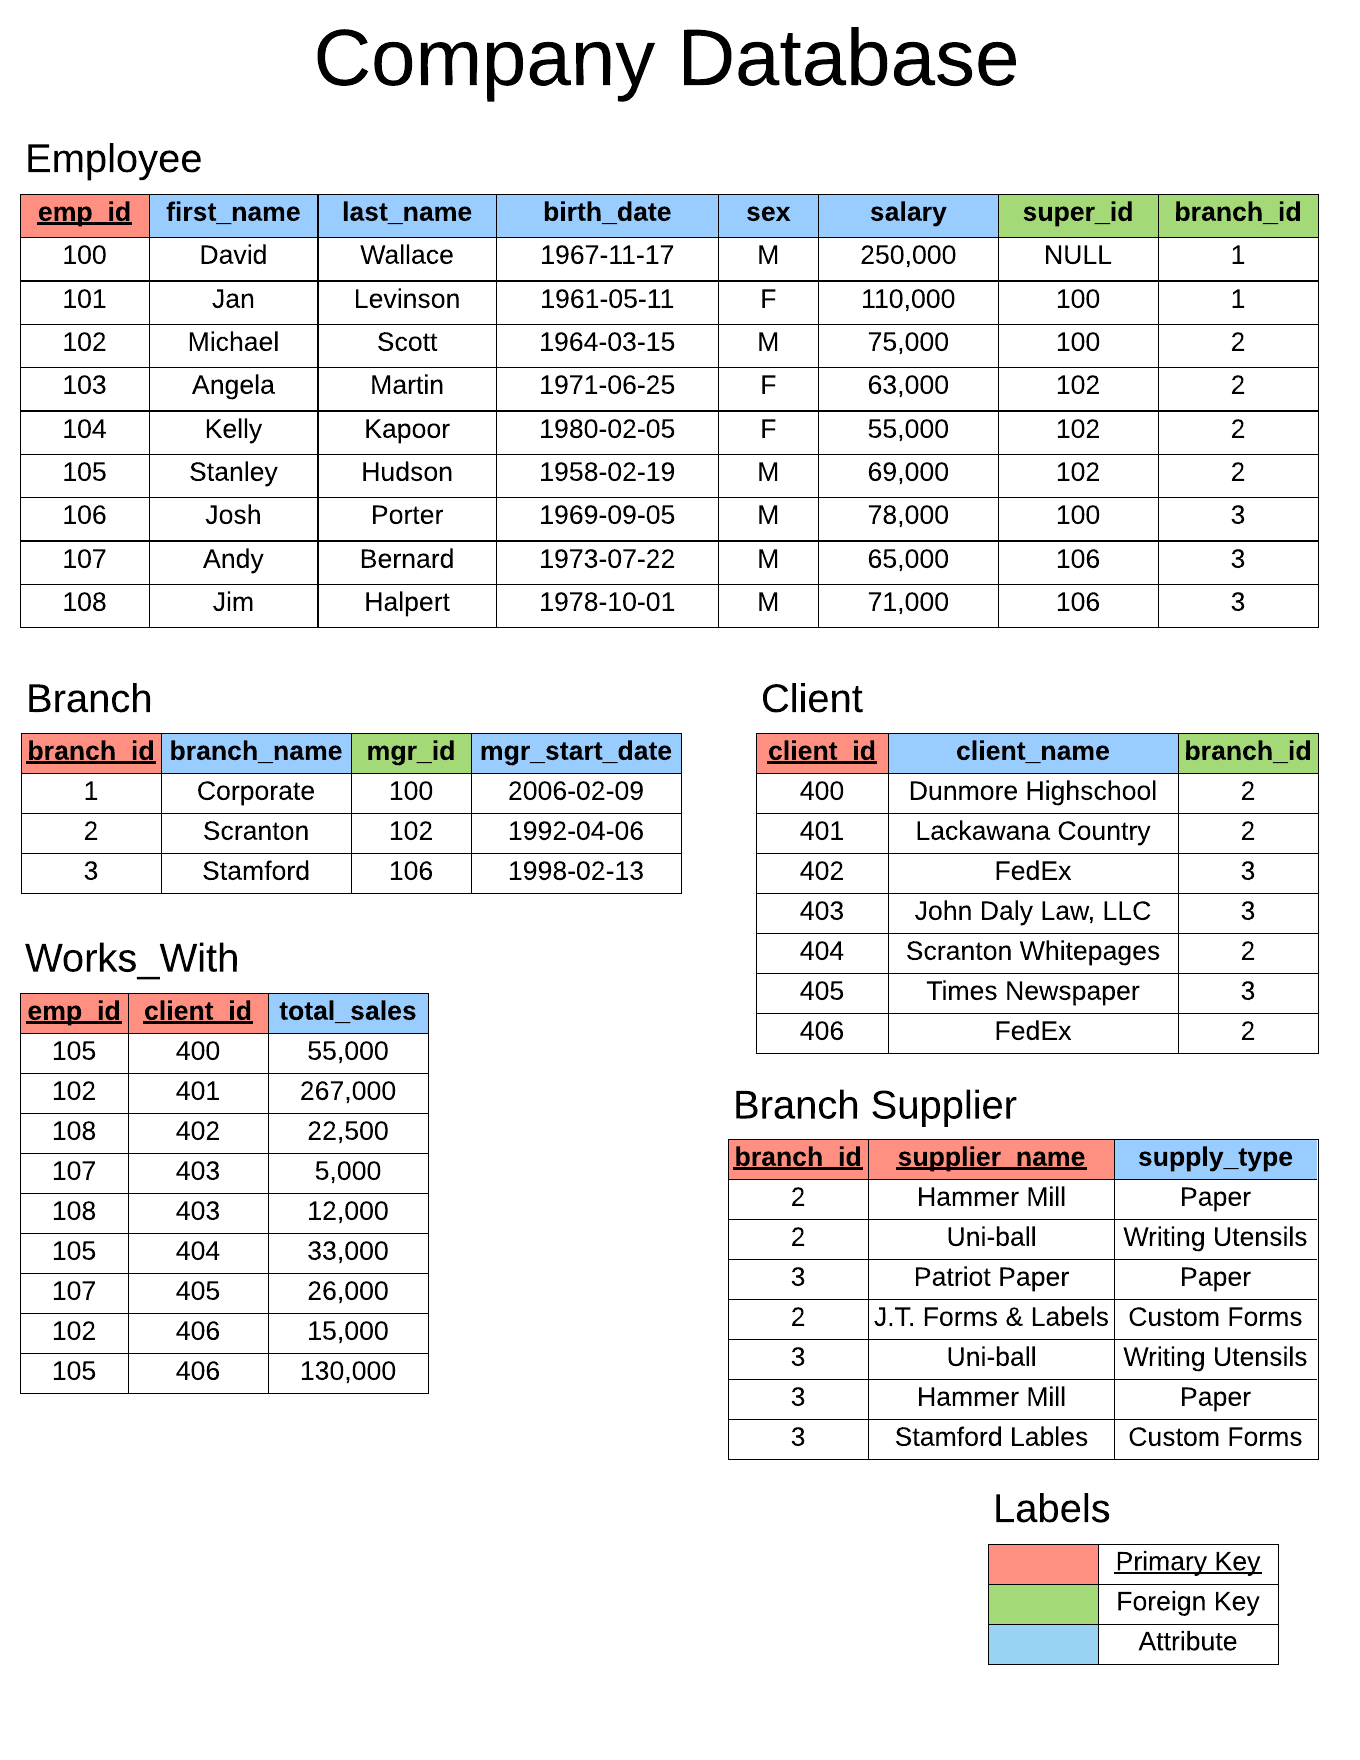
\includegraphics[width=0.5\textwidth,height=0.5\textheight,keepaspectratio]{company-database}
\begin{minted}{SQL}
CREATE TABLE employee (
  emp_id INT PRIMARY KEY,
  first_name VARCHAR(40),
  last_name VARCHAR(40),
  birth_day DATE,
  sex VARCHAR(1),
  salary INT,
  super_id INT,
  branch_id INT
);

CREATE TABLE branch (
  branch_id INT PRIMARY KEY,
  branch_name VARCHAR(40),
  mgr_id INT,
  mgr_start_date DATE,
  FOREIGN KEY(mgr_id) REFERENCES employee(emp_id) ON DELETE SET NULL
  -- example of multiple foreign key:
  -- foreign key (course_id, sec_id, semester) references section (course_id, sec_id, semester) on delete cascade
  -- foreign key (ID) references student (ID) on delete cascade
);

ALTER TABLE employee
ADD FOREIGN KEY(branch_id)
REFERENCES branch(branch_id)
ON DELETE SET NULL;

ALTER TABLE employee
ADD FOREIGN KEY(super_id)
REFERENCES employee(emp_id)
ON DELETE SET NULL;

CREATE TABLE client (
  client_id INT PRIMARY KEY,
  client_name VARCHAR(40),
  branch_id INT,
  FOREIGN KEY(branch_id) REFERENCES branch(branch_id) ON DELETE SET NULL
);

CREATE TABLE works_with (
  emp_id INT,
  client_id INT,
  total_sales INT,
  PRIMARY KEY(emp_id, client_id),  -- in this way we can set multiple primary keys.
  FOREIGN KEY(emp_id) REFERENCES employee(emp_id) ON DELETE CASCADE,
  FOREIGN KEY(client_id) REFERENCES client(client_id) ON DELETE CASCADE
);

CREATE TABLE branch_supplier (
  branch_id INT,
  supplier_name VARCHAR(40),
  supply_type VARCHAR(40),
  PRIMARY KEY(branch_id, supplier_name),
  FOREIGN KEY(branch_id) REFERENCES branch(branch_id) ON DELETE CASCADE
);


-- -----------------------------------------------------------------------------

-- Corporate
INSERT INTO employee VALUES(100, 'David', 'Wallace', '1967-11-17', 'M', 250000, NULL, NULL);

INSERT INTO branch VALUES(1, 'Corporate', 100, '2006-02-09');

UPDATE employee
SET branch_id = 1
WHERE emp_id = 100;

INSERT INTO employee VALUES(101, 'Jan', 'Levinson', '1961-05-11', 'F', 110000, 100, 1);

-- Scranton
INSERT INTO employee VALUES(102, 'Michael', 'Scott', '1964-03-15', 'M', 75000, 100, NULL);

INSERT INTO branch VALUES(2, 'Scranton', 102, '1992-04-06');

UPDATE employee
SET branch_id = 2
WHERE emp_id = 102;

INSERT INTO employee VALUES(103, 'Angela', 'Martin', '1971-06-25', 'F', 63000, 102, 2);
INSERT INTO employee VALUES(104, 'Kelly', 'Kapoor', '1980-02-05', 'F', 55000, 102, 2);
INSERT INTO employee VALUES(105, 'Stanley', 'Hudson', '1958-02-19', 'M', 69000, 102, 2);

-- Stamford
INSERT INTO employee VALUES(106, 'Josh', 'Porter', '1969-09-05', 'M', 78000, 100, NULL);

INSERT INTO branch VALUES(3, 'Stamford', 106, '1998-02-13');

UPDATE employee
SET branch_id = 3
WHERE emp_id = 106;

INSERT INTO employee VALUES(107, 'Andy', 'Bernard', '1973-07-22', 'M', 65000, 106, 3);
INSERT INTO employee VALUES(108, 'Jim', 'Halpert', '1978-10-01', 'M', 71000, 106, 3);


-- BRANCH SUPPLIER
INSERT INTO branch_supplier VALUES(2, 'Hammer Mill', 'Paper');
INSERT INTO branch_supplier VALUES(2, 'Uni-ball', 'Writing Utensils');
INSERT INTO branch_supplier VALUES(3, 'Patriot Paper', 'Paper');
INSERT INTO branch_supplier VALUES(2, 'J.T. Forms & Labels', 'Custom Forms');
INSERT INTO branch_supplier VALUES(3, 'Uni-ball', 'Writing Utensils');
INSERT INTO branch_supplier VALUES(3, 'Hammer Mill', 'Paper');
INSERT INTO branch_supplier VALUES(3, 'Stamford Lables', 'Custom Forms');

-- CLIENT
INSERT INTO client VALUES(400, 'Dunmore Highschool', 2);
INSERT INTO client VALUES(401, 'Lackawana Country', 2);
INSERT INTO client VALUES(402, 'FedEx', 3);
INSERT INTO client VALUES(403, 'John Daly Law, LLC', 3);
INSERT INTO client VALUES(404, 'Scranton Whitepages', 2);
INSERT INTO client VALUES(405, 'Times Newspaper', 3);
INSERT INTO client VALUES(406, 'FedEx', 2);

-- WORKS_WITH
INSERT INTO works_with VALUES(105, 400, 55000);
INSERT INTO works_with VALUES(102, 401, 267000);
INSERT INTO works_with VALUES(108, 402, 22500);
INSERT INTO works_with VALUES(107, 403, 5000);
INSERT INTO works_with VALUES(108, 403, 12000);
INSERT INTO works_with VALUES(105, 404, 33000);
INSERT INTO works_with VALUES(107, 405, 26000);
INSERT INTO works_with VALUES(102, 406, 15000);
INSERT INTO works_with VALUES(105, 406, 130000);

-- Find out all the different genders
-- SQL allows duplication in query results.
-- can use distinct to force elimination.
-- if we would have used select sex, then it would have shown all rows under attribute sex under relation employee.
SELECT DISTINCT sex
FROM employee;

-- Find the total number of instructors who teach a course in the Spring 2010
semester
select count (distinct ID)
from teaches
where semester = ’Spring’ and year = 2010;

-- find the no. of tuples in course relation
select count(*) from course;

-- Find names of instructors with salary greater than that of some (at least one)
-- instructor in the Biology department.
select distinct T.name
from instructor as T, instructor as S
where T.salary > S.salary and S.dept name = ’Biology’;

-- same query using some clause

select name
from instructor
where salary > some (select salary
from instructor
where dept name = ’Biology’);

-- Find all employee's id's and names who were born after 1969
SELECT emp_id, first_name, last_name
FROM employee
WHERE birth_day >= 1970-01-01;

-- Find all employees born between 1970 and 1975
SELECT *
FROM employee
WHERE birth_day BETWEEN '1970-01-01' AND '1975-01-01';

-- Functions

-- Find the number of employees
SELECT COUNT(super_id)
FROM employee;

-- Find the average of all employee's salaries
SELECT AVG(salary)
FROM employee;

-- Find the names and average salaries of all departments whose average salary is
-- greater than 42000

select dept_name, avg (salary)
from instructor
group by dept_name
having avg (salary) > 42000;

-- predicates in the having clause are applied after the
-- formation of groups whereas predicates in the where
-- clause are applied before forming groups

-- Delete all instructors whose salary is less than the average salary of instructors

delete from instructor
where salary < (select avg (salary)
from instructor);

-- Problem: as we delete tuples from deposit, the average salary
-- changes but its not an issue with mysql/mariadb.

-- Find the sum of all employee's salaries
SELECT SUM(salary)
FROM employee;

-- Aggregation.
-- Find out how many males and females there are
SELECT COUNT(sex), sex  -- now we have two columns, viz, COUNT(sex) and sex.
FROM employee
GROUP BY sex

-- Find the total sales of each salesman
SELECT SUM(total_sales), emp_id
FROM works_with
GROUP BY emp_id;
-- IMP NOTE: sum does not avoid null values, null + something is always null so better check for null values. Actually result of any arithmetic expression involving null is null.
-- Need to confirm the above point as in slides it is mentioned that all aggregate operations except count (*) ignore tuples will null values on the aggregate attributes.
-- And according to slides, if the collection has only null values then 
-- • count returns 0
-- • count(*) return number of rows with null values
-- • all other aggregates return null

select sum(tot_cred) from student where tot_cred is not null;
-- if we want to check for null we could have written "is null" instead of "is not null".

-- Find the total amount of money spent by each client
SELECT SUM(total_sales), client_id
FROM works_with
GROUP BY client_id;

select dept_name from department, (select max(budget) as MX from department) as T where budget = T.MX;

select dept_name, max(AG) from (select dept_name, avg(salary) as AG from instructor group by dept_name) as M;

select name, salary, dept_name from instructor where salary > all (select salary from instructor where dept_name in ('Biology', 'History', 'Finance'));

-- Wildcards

-- % = any # characters, _ = one character

-- Find any employee born on the 10th day of the month
SELECT *
FROM employee
WHERE birth_day LIKE '_____10%';

-- Match the string '100%'
like '100 \%' escape '\'
-- in above we use backslash (\) as the escape character.

-- Find any clients who are schools
SELECT *
FROM client
WHERE client_name LIKE '%Highschool%';

-- Union 

-- Find a list of all clients & branch suppliers' names
SELECT client.client_name AS Non-Employee_Entities, client.branch_id AS Branch_ID
FROM client
UNION -- both above and below thing should have same number of columns and same data type respectively
SELECT branch_supplier.supplier_name, branch_supplier.branch_id
FROM branch_supplier;

-- Just like union with same rules we have INTERSECT and EXCEPT and each of them automatically eliminates duplicates that is it inherently assumes DISTINCT. To retain all duplicates use the corresponding multiset versions union all, intersect all, except all (in maria db all is not supported with intersect).

-- Suppose a tuple occurs m times in r and n times in s, then, it occurs:
-- • m + n times in r union all s
-- • min(m,n) times in r intersect all s
-- • max(0, m – n) times in r except all s

-- Exist and not exist
-- exists r iff r != phi
-- not exists r iff r == phi

-- Yet another way of specifying the query “Find all courses taught in both the Fall 2009 semester and in the Spring 2010 semester”

select course_id
from section as S
where semester = ’Fall’ and year = 2009 and
exists (select *
from section as T
where semester = ’Spring’ and year= 2010
and S.course_id = T.course_id);

-- Find all students who have taken all courses offered in the Biology department

select distinct S.ID, S.name
from student as S
where not exists ( (select course_id
from course
where dept_name = ’Biology’)
except
(select T.course_id
from takes as T
where S.ID = T.ID));

-- The unique construct tests whether a subquery has any duplicate tuples in its
result.
-- The unique construct evaluates to “true” if a given subquery contains no duplicates.
-- Find all courses that were offered at most once in 2009
select T.course_id
from course as T
where unique (select R.course_id
from section as R
where T.course_id= R.course_id
and R.year = 2009);

-- With
-- The with clause provides a way of defining a temporary relation whose definition is
-- available only to the query in which the with clause occurs.
-- Find all departments with the maximum budget

with max_budget (value) as
(select max(budget)
from department)
select department.name
from department, max_budget
where department.budget = max_budget.value;

-- Find all departments where the total salary is greater than the average
of the total salary at all departments

with dept _total (dept_name, value) as
(select dept_name, sum(salary)
from instructor
group by dept_name),
dept_total_avg(value) as
(select avg(value)
from dept_total)
select dept_name
from dept_total, dept_total_avg
where dept_total.value > dept_total_avg.value;

-- JOINS (used to combine rows from two or more tables based on the related columns) (Simply using 'join' then 'on' means that we are using inner join)
-- In book it is written natural join where we don't have to specify "on". Also we have natural left/right/full outer join. (notice the word outer). If we dont use natural then we would have to write left/right/full outer join .. on <condition>
-- Similarly in our normal join instead of writing "on" or "natural", we can write using <A1, A2, ..., Ak>
-- IMP NOTE: 
select *
from student left outer join takes on student.ID= takes.ID;
-- is different from 
select *
from student left outer join takes on true
where student.ID= takes.ID;
-- The earlier query, using the left outer join with the on condition, includes a tuple
-- (70557, Snow, Physics, 0, null, null, null, null, null, null ), because there is no tuple
-- in takes with ID = 70557. In the latter query, however, every tuple satisfies the join
-- condition true, so no null-padded tuples are generated by the outer join. The outer
-- join actually generates the Cartesian product of the two relations. Since there is
-- no tuple in takes with ID = 70557, every time a tuple appears in the outer join with
-- name = “Snow”, the values for student.ID and takes.ID must be different, and such
-- tuples would be eliminated by the where clause predicate. Thus student Snow
-- The earlier query, using the left outer join with the on condition, includes a tuple
-- (70557, Snow, Physics, 0, null, null, null, null, null, null ), because there is no tuple
-- in takes with ID = 70557. In the latter query, however, every tuple satisfies the join
-- condition true, so no null-padded tuples are generated by the outer join. The outer
-- join actually generates the Cartesian product of the two relations. Since there is
-- no tuple in takes with ID = 70557, every time a tuple appears in the outer join with
-- name = “Snow”, the values for student.ID and takes.ID must be different, and such
-- tuples would be eliminated by the where clause predicate. Thus student Snow
-- never appears in the result of the latter query.never appears in the result of the latter query.

-- Add the extra branch
INSERT INTO branch VALUES(4, "Buffalo", NULL, NULL);  -- here I have used double quotes but strings can as well be represented with single quotes.

-- Find all branches and the names of their managers
SELECT employee.emp_id, employee.first_name, branch.branch_name
FROM employee
JOIN branch    -- LEFT JOIN (when we use LEFT JOIN all the rows from the left table gets included as well, similarly for RIGHT JOIN), RIGHT JOIN  (we added buffalo just so that we can see difference in case of RIGHT JOIN)
ON employee.emp_id = branch.mgr_id;
-- we can add a where clause beneath this like where branch.mgr_start_date > something

-- Show ID, name, courses, and corresponding credits of each student.
select M.ID, M.name, C.title, C.credits from (select S.ID, S.name, T.course_id from student as S join takes as T on S.ID = T.ID) as M join course as C on M.course_id = C.course_id;

-- nested queries

-- Find names of all employees who have sold over 50,000
SELECT employee.first_name, employee.last_name
FROM employee
WHERE employee.emp_id IN (SELECT works_with.emp_id  -- note that first sql will execute the part which is inside "()"
                          FROM works_with
                          WHERE works_with.total_sales > 50000);

-- Find all clients who are handled by the branch that Michael Scott manages
-- Assume you know Michael's ID
SELECT client.client_id, client.client_name
FROM client
WHERE client.branch_id = (SELECT branch.branch_id
                          FROM branch
                          WHERE branch.mgr_id = 102);

 -- Find all clients who are handles by the branch that Michael Scott manages
 -- Assume you DONT'T know Michael's ID
 SELECT client.client_id, client.client_name
 FROM client
 WHERE client.branch_id = (SELECT branch.branch_id
                           FROM branch
                           WHERE branch.mgr_id = (SELECT employee.emp_id
                                                  FROM employee
                                                  WHERE employee.first_name = 'Michael' AND employee.last_name ='Scott'
                                                  LIMIT 1));


-- Find the names of employees who work with clients handled by the scranton branch
SELECT employee.first_name, employee.last_name
FROM employee
WHERE employee.emp_id IN (
                         SELECT works_with.emp_id
                         FROM works_with
                         )
AND employee.branch_id = 2;

-- Find the names of all clients who have spent more than 100,000 dollars
SELECT client.client_name
FROM client
WHERE client.client_id IN (
                          SELECT client_id
                          FROM (
                                SELECT SUM(works_with.total_sales) AS totals, client_id
                                FROM works_with
                                GROUP BY client_id) AS total_client_sales
                          WHERE totals > 100000
);

-- Correct the tot_credit attributes for each tuple in student table such that total credit is
equal to the credit of courses successfully completed by the student. Here successfully
completed means student has a grade that is not ‘F’ . Students who did not take any
courses, the output for them should show total credit 0.

update student as ST, (select B.ID, coalesce(B.crd, 0) as cred from (select J.ID, sum(C.credits) as crd from (select N.ID, N.grd, N.course_id from (select M.ID, coalesce(M.grade, 'N') as grd, M.course_id from (select S.ID, S.name, T.course_id, T.grade from student as S left join takes as T on S.ID = T.ID) as M) as N) as J left join course as C on J.course_id = C.course_id where J.grd <> 'F' group by J.ID) as B) as TEMP set tot_cred = TEMP.cred where ST.ID = TEMP.ID;

-- Maybe it could have been done like this

update student S
set tot_cred = (select sum(credits)
from takes, course
where takes.course_id = course.course_id and
S.ID= takes.ID.and
takes.grade <> ’F’ and
takes.grade is not null);

-- Sets tot_creds to null for students who have not taken any course
-- Instead of sum(credits), use:

case
when sum(credits) is not null then sum(credits)
else 0
end

-- deleting entries in the table when they have foreign keys associated to them
-- ON DELETE NULL means that say if we delete Michael Scott then second entry in the branch table will get mgr_id set to NULL whereas in ON DELETE CASCADE the entire row will get deleted in branch table. Use ON DELETE CASCADE when that foreign key is very important like say it forms a primary key.
-- If you set the relation ship to be ON DELETE CASCADE, when you run a DELETE statement on a parent table it will DELETE all the corresponding rows from the CHILD table automatically. But the RESTRICT (which is the default foreign key relationship behavior) is when you try to delete a row from the parent table and there is a row in the child table with the same ID, it will fail complaining about the existing child rows.
-- Similarly we could have done on update cascade, on delete set null/default

-- Views
-- SQL allows a “virtual relation” to be defined by a query, and the
-- relation conceptually contains the result of the query. The virtual relation is not
-- precomputed and stored, but instead is computed by executing the query whenever the virtual relation is used. Thus if table changes, view changes.
-- Any such relation that is not part of the logical model, but is made visible to a user as a virtual relation, is called a view

-- Create view of students who are studying in a department with budget more than 80000

create view stud_dept_budg as select S.ID, S.name, S.dept_name, D.budget from student as S join department as D on S.dept_name = D.dept_name where D.budget > 80000;

-- Now if we delete (or dec budget) some department with budget > 80000. and then do select * from stud_dept_budg; it wont show name corresponding to that department.
-- We can now also do select building from stud_dept_budg where <something>

-- One view may be used in the expression defining another view. For example,
-- we can define a view physics fall 2009 watson that lists the course ID and room
-- number of all Physics courses offered in the Fall 2009 semester in the Watson
-- building as follows:
-- create view physics fall 2009 watson as
-- select course id, room number
-- from physics_fall_2009  -- Note that this physics_fall_2009 is inturn a view
-- where building= ’Watson’;
-- 
-- Certain database systems allow view relations to be stored, but they make sure
-- that, if the actual relations used in the view definition change, the view is kept
-- up-to-date. Such views are called materialized views.
-- The process of keeping the materialized view up-to-date is called materialized view maintenance (or often, just view maintenance) 
-- 
-- Updates on view are generally tough to implement and hence isn't much supported by database systems

-- CREATE
--     TRIGGER `event_name` BEFORE/AFTER INSERT/UPDATE/DELETE
--     ON `database`.`table`
--     FOR EACH ROW BEGIN
-- 		-- trigger body
-- 		-- this code is applied to every
-- 		-- inserted/updated/deleted row
--     END;

CREATE TABLE trigger_test (
     message VARCHAR(100)
);


DELIMITER $$  -- changing delimiter from semicolon to $$ as we will be using semicolon inside and we don't want sql to think that when we put semicolon we are done with our trigger
CREATE
    TRIGGER my_trigger BEFORE INSERT
    ON employee
    FOR EACH ROW BEGIN  -- for each new item that is inserted
        INSERT INTO trigger_test VALUES('added new employee');
    END$$
DELIMITER ;  -- changing delimiter back to semi colon.
INSERT INTO employee
VALUES(109, 'Oscar', 'Martinez', '1968-02-19', 'M', 69000, 106, 3);


DELIMITER $$
CREATE
    TRIGGER my_trigger BEFORE INSERT
    ON employee
    FOR EACH ROW BEGIN
        INSERT INTO trigger_test VALUES(NEW.first_name);
    END$$
DELIMITER ;
INSERT INTO employee
VALUES(110, 'Kevin', 'Malone', '1978-02-19', 'M', 69000, 106, 3);

DELIMITER $$
CREATE
    TRIGGER my_trigger BEFORE INSERT
    ON employee
    FOR EACH ROW BEGIN 
         IF NEW.sex = 'M' THEN
               INSERT INTO trigger_test VALUES('added male employee');
         ELSEIF NEW.sex = 'F' THEN
               INSERT INTO trigger_test VALUES('added female');
         ELSE
               INSERT INTO trigger_test VALUES('added other employee');
         END IF;
    END$$
DELIMITER ;
INSERT INTO employee
VALUES(111, 'Pam', 'Beesly', '1988-02-19', 'F', 69000, 106, 3);


DROP TRIGGER my_trigger;
\end{minted}
Around last 20 mins of that video show how to convert ER Diagram to actual database schema.

Entity = An object we want to model and store information about

Attributes = Specific pieces of information about an entity

Composite attribute = An attribute that can be broken up into sub attributes

Multi - valued attribute = An attribute than can have more than one value (like same student can have more than one club but only one GPA)

Derived Attribute = An attribute that can be derived from the other attributes.

ER = Entity Relationship defines a relationship between two entities.

Relationship Attribute = An attribute about the relationship

\subsection{Lect1}
Levels of abstraction

Physical level: describes how a record (e.g., instructor) is stored.

Logical level: describes data stored in database, and the relationships among 
the data.

View level: application programs hide details of data types.  Views can also 
hide information (such as an employee’s salary) for security purposes. 

Logical Schema: the overall logical structure of the database 
Example: The database consists of information about a set of customers and 
accounts in a bank and the relationship between them
Analogous to type information of a variable in a program

Physical schema: the overall physical structure of the database 

Instance: the actual content of the database at a particular point in time 
Analogous to the value of a variable

Physical Data Independence: the ability to modify the physical schema without 
changing the logical schema

Data Models: A collection of tools for describing Data, Data relationships, Data semantics, Data constraints. Ex: Relationship Model, Entity relationship model, object based model.

Database engine: 

1) Storage manager: is a program module that provides the interface between 
the low-level data stored in the database and the application programs and 
queries submitted to the system.

2) Query Processing

3) Transaction Management:- 

A transaction consists of a sequence of query and/or update statements.
Commit work commits the current transaction; that is, it makes the updates
performed by the transaction become permanent in the database. After the
transaction is committed, a new transaction is automatically started.
Rollback work causes the current transaction to be rolled back; that is, it
undoes all the updates performed by the SQL statements in the transaction.
Thus, the database state is restored to what it was before the first statement
of the transaction was executed.
Once a transaction has executed commit work, its
effects can no longer be undone by rollback work. The database system guarantees that in the event of some failure, such as an error in one of the SQL statements,
a power outage, or a system crash, a transaction’s effects will be rolled back if it
has not yet executed commit work
Transaction: is a collection of operations that performs a single 
logical function in a database application

Transaction-management component: ensures that the database 
remains in a consistent (correct) state despite system failures (e.g., 
power failures and operating system crashes) and transaction failures.
\subsection{Lect2}
Lecture was about relational model

K is a superkey of R if values for K are sufficient to identify a unique tuple of each possible relation r of R.

Superkey K is a candidate key if K is minimal

One of the candidate key is selected to be the primary key
\subsection{Lect3}
An entity is a “thing” or “object” in the real world that is 
distinguishable from other objects. 

Entities are described in a database by a set of attributes

A relationship is an association among several entities

The set of all entities of the same type and the set of all relationships of the same type are termed an entity set and relationship set, respectively. 

A relationship may also have attributes called descriptive attributes

Domain: the set of permitted values for each attribute 

An entity set that does not have sufficient attributes to form a primary key is termed a weak entity set

An entity set that has a primary key is termed a strong entity set

For a weak entity set to be meaningful, it must be associated with another entity set, called the identifying or owner entity set

Every weak entity must be associated with an identifying entity; that is, the weak entity set is said to be existence dependent on the  identifying entity set. The identifying entity set is said to  own the  weak entity set that it identifies. 

The relationship associating the weak entity set with the identifying  entity set is called the identifying relationship

The discriminator (or partial key) of a weak entity set is the set of attributes that distinguishes among all the entities of a weak entity set.

The primary key of a weak entity set is formed by the primary key of the strong entity set on which the weak entity set is existence dependent, plus the weak entity set’s discriminator
\subsection{Lect4-5}
See slides.
\subsection{Lect6}
See slides.
\subsection{Lect7-9}
In slide, see slide: 25, 26, 31
\subsection{Lect10}
Nothing. All incorporated into this notes.
\end{document}